\documentclass[../main.tex]{subfiles}
\graphicspath{{\subfix{../figures/}}}
%
\begin{document}
\section{代理模式(proxy)}
\noindent 代理模式给某一个对象提供一个代理,并由代理对象控制对原对象的引用.

代理模式的英文为Proxy,中文可译成“代理”.所谓代理,就是一个人或者一个机构代表另一个人或者另一个机构采取行动.在一些情况下,一个客户端对象不想或者不能够直接引用一个对象,而代理对象可以在客户端和目标对象之间起到中介的作用.
%
\begin{figure}[H]
  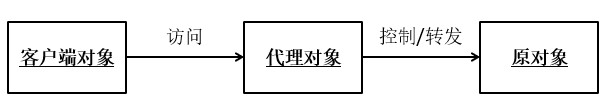
\includegraphics[width=0.35\textwidth]{23_1.jpg}
\end{figure}
%
\textbf{若按使用目的划分,代理有以下几种}:
\begin{itemize}
  \item 远程(Remote)代理:为一个位于不同的地址空间的对象提供一个局域代理对象.这个不同的地址空间可以是在本机器中,也可是在另一台机器中.远程代理又叫做大使(Ambassador).
  \item 虚拟(Virtual)代理:根据需要创建一个资源消耗较大的对象,使得此对象只在需要时才会被真正创建.
  \item Copy-on-Write代理:虚拟代理的一种.把复制(克隆)拖延到只有在客户端需要时,才真正采取行动.
  \item 保护(Protect or Access)代理:控制对一个对象的访问,如果需要,可以给不同的用户提供不同级别的使用权限.
  \item Cache代理:为某一个目标操作的结果提供临时的存储空间,以便多个客户端可以共享这些结果.
  \item 防火墙(Firewall)代理:保护目标,不让恶意用户接近.
  \item 同步化(Synchronization)代理:使几个用户能够同时使用一个对象而没有冲突.
\end{itemize}
%
\textbf{代理的例子} :
Windows系统提供快捷方式(Shortcut),可以使任何对象同时出现在多个地方而不必修改原对象.对快捷方式的调用完全与对原对象的调用一样,换言之,快捷方式对客户端是完全透明的.
%
\subsection{代理模式的结构}
代理模式的类图如图所示:
%
\begin{figure}[H]
  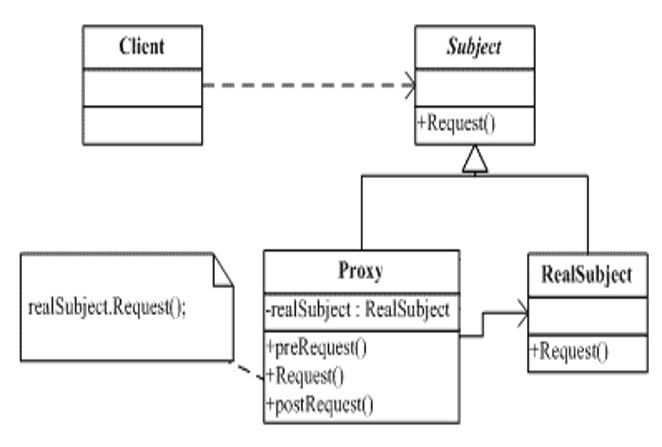
\includegraphics[width=0.45\textwidth]{23_2.jpg}
\end{figure}
%
\textbf{代理模式所涉及的角色}:
\begin{itemize}
  \item 抽象主体角色(Subject):声明了真实主体和代理主体的共同接口,这样一来在任何使用真实主体的地方都可以使用代理主体.
  \item 代理主体(Proxy)角色:代理主体角色内部含有对真实主体的引用,从而可以在任何时候操作真实主体对象;代理主体角色提供一个与真实主体角色相同的接口,以便可以在任何时候都可以替代真实主体;控制真实主体的引用,负责在需要的时候创建真实主体对象(和删除真实主体对象);代理角色通常在将客户端调用传递给真实的主体之前或之后,都要执行某个操作,而不是单纯的将调用传递给真实主体对象.
  \item 真实主体角色(RealSubject)角色:定义了代理角色所代表的真实对象.
\end{itemize}
%
\lstinputlisting[language=java]{./code/23/1/Subject.java}
\lstinputlisting[language=java]{./code/23/1/RealSubject.java}
\lstinputlisting[language=java]{./code/23/1/ProxySubject.java}
%
调用代理主体: \\
\texttt{Subject subject=new ProxySubject();subject.request();}
\end{document}
